% Chapter 7

\chapter{Literature Review} % Main chapter title

\label{Chapter7_literature-review} % For referencing the chapter elsewhere, use \ref{Chapter7} 

\section{Introduction }
This chapter is answer to the sub research question 1. 
In this chapter, first mention 
is about the literature search approach 
and then a literature review was done to understand the current state of available artefacts according to the literature. 
It helped to find the gaps between the available artefacts 
and the desirable artefacts. 

From the collected academic work, 
the existing knowledge on cyber newsfeed assessment process 
and related concepts like people, practices, 
guidelines and methods available according to academic literature 
(sub research question 1a) are listed. 
It also illuminate about the vendor field of automated cyber newsfeed suppliers of the artefacts (sub research question 1b).  
Collected literature has been used to explore the following topics.

\begin{enumerate}
    \item Existing practices, systems, and people involved in automated cyber newsfeed.
   
    \item Existing guidelines on cyber newsfeeds correlation, contextualization, and analytics. 
    
     \item Existing methods available for data source quality assessment.
\end{enumerate}

\section{Approach}

I have searched the knowledge body in different sources and some knowledge was acquired during the discussion with ON2IT cybersecurity professionals. 
The primary sources of knowledge included academic publications, textbooks, research papers in journals and conferences. The additional sources of knowledge exploration were online magazine articles, white papers, websites, and artefact manuals. 
Exclusive details about the publication year criteria, used keywords and the libraries are listed below.
\begin{enumerate}
    \item  Filter on \textbf{year greater than 2010} to make it relevant.
    \item  The important keywords used for the search used 
        \textbf{cyber, security, threat, news, intelligence, live, RSS, news, feed, system, artefact, people, cyber experts, information, intel} or \textbf{feeds}.
    \item  Libraries used for academic papers: \textbf{Google Scholar} and \textbf{Web of Science}.
    \item  Search String formulation:\textbf{cyber +(security|threat|news|intelligence) + [(live|rss|news)]+ [Feed[s]]}.

\end{enumerate}

The above search string will follow the following match pattern shown as an example in the TABLE \ref{tab:search-pattern}.



\begin{table}
    \caption{Illustration of search pattern: Literature Search Analogy}
    \label{tab:search-pattern}
    \centering{}
   \resizebox{\textwidth}{!}{
    \begin{tabular}{|l|l|l|l|}
    \toprule
      \rowcolor[HTML]{BFCEED} 
    \textbf{Symbol} & \textbf{Meaning X} & \textbf{Example } & \textbf{Interpretation} \\
    \midrule
    {[]} & Zero or One Occurrence of the string or character within square bracket & [Feed] & “Feed” or null \\
    {[ ]} & Zero or One Occurrence of the string or character within square bracket & [s] & “s” or null\\
    ( ) & One Occurrence & (Security) & Security \\
    | & Optional & live|rss & either “live” or “rss”\\
    + & And & cyber + security & “cyber” and “Security” both \\
    \bottomrule
    \end{tabular}
}
\end{table}

\section{Overview of the literature search}
I explored 52 papers using snowball \citep{wohlin2014guidelines} approach and the majority of those papers are re-used and lined up in  bibliograpy \ref{sec:bibliography}. 



\section{Existing practices, systems, and people involved in automated cyber newsfeed}\label{Existing practices, systems, and people involved in automated cyber newsfeed}


In this section the existing literature about the practices, systems and people involved has been covered to explain the existing environment in which cybersecurity world and cyber newsfeed are interrelated. 
The first section \ref{Existing-practices}, \nameref{Existing-practices} deals with the generic practices involved in cybersecurity world and how cyber newsfeed is important to such practices in cybersecurity world. 
The second section \ref{Existing systems}, \nameref{Existing systems} and third  section \ref{People}, \nameref{People}  deal with the relation and importance of systems and people involved in cyber security world and how is cyber newsfeed is importance to them. 

\cite{sector10itu} states that cybersecurity is the collection of tools, policies, security concepts, security safeguards, guidelines, risk management approaches, actions, training, best practices, assurance and technologies that can be used to protect the cyber environment and organization and user’s assets. 

Organization and user’s assets include connected computing devices, personnel, infrastructure, applications, services, telecommunications systems, and the totality of transmitted and/or stored information in the cyber environment.

Cybersecurity strives to ensure the attainment and maintenance of the security properties of the organization and user’s assets against relevant security risks in the cyber environment 
\citep{sector10itu}. 
The general security objectives comprise the following: Availability Integrity, which may include authenticity and non repudiation Confidentiality 
\citep{sector10itu}.



\subsection{Existing practices}\label{Existing-practices}

With the rapid growth in use of Information Technology, organizations are getting very vigilant when it comes to protecting business information. Form simple security solutions (e.g., anti-virus software and firewalls) to complex security solution (e.g., 3G\footnote{3G or Application firewall \url{http://www.avolio.com/papers/FWTKv1.0Announcement.html}} firewalls), organizations are doing the best possible security investment and management \citep{yeh2007threats}. 
At the same time the cyber attackers are continuously trying to invent new ways of attacking IT systems and their approach to attack vulnerabilities has also evolved over time \citep{jang2014survey}. 

This means that as an organization, one cannot ensure 100 percent guarantee of secure IT systems. Despite putting a lot of effort on safeguarding and securing organizational assets, there are high chances of getting exposed to any unpredictable security incident. In such unpredictable situations, to avoid cyber security incidents, keeping an eye on daily updates happening in dark web is very important \citep{chen2006intelligence}. 
Such cyber information related about information security, new threats, vulnerabilities, security products, and research is available on internet with open access \citep{fogelman2008mining}. These information can be used in many ways and
 \cite{zimmerman2014ten} provides 10 strategies to handle such cyber information.

\begin{itemize}
    \item \textbf{Cyber Intel Collection:} Collection and consumption of cyber intelligence reports, cyber intrusion reports, and news related to information security, covering new threats, vulnerabilities, products, and research. 
    
    \item \textbf{Cyber Intel Analysis:} Analysis is done manually by security analysts or by automatically by some security vendors, in some organization they use in house cyber news analytics system.

    \item \textbf{Cyber Intel Distribution:} Post analysis redistribution of cyber intelligence reports, cyber intrusion reports, and news related to information security to members on either a routine basis such as a weekly or monthly cyber newsletter or a non-routine basis such as an emergency patch notice or phishing campaign alert. 
    
    \item \textbf{Cyber Intel Creation:} In case of newly observed threat based on primary research analysis of a new threat or vulnerability, the result of research is shared with larger audience of potential beneficiaries.
    
    \item \textbf{Cyber Intel Fusion:} Extracting data from cyber intel and synthesizing it into new signatures, content, and understanding of adversary Search Results. Tactics, Techniques and Procedures (TTPs), thereby evolving monitoring operations 
    (e.g., new signatures or Security Information and Event Management (SIEM) content). 
    
    \item \textbf{Trending:} Long-term analysis of event feeds, collected malware, and incident data for evidence of malicious or anomalous activity or to better understand the constituency or adversary. For analogy any information on phishing email about COVID-19 and privacy concern in online meeting tools were trending during Feb-2020 to Apr-2020. 

    \item \textbf{Cyber Threat Assessment:} An estimation of potential threats on existing IT systems. This is often performed in coordination with other cybersecurity stakeholders. 
\end{itemize}

\subsection{Existing systems for Cyber Intelligence Sharing}\label{Existing systems}
This section is about the explored systems, according to existing literature which are associated with cyber newsfeed collection, processing and production. 
A generic term for such systems would be \textbf{Cyber Threat Intelligence Sharing Platforms}.
These systems when used in practice provides operational mechanisms to support the exchange of intelligence on cyber security threats and incidents amongst different entities \citep{brown2015cyber,sauerwein2018shadow}.  The related systems types has been presented here below is based on 1) Systems producing or publishing cyber newsfeed on Internet and 2) Systems consuming or collecting cyber newsfeed from Internet.

\begin{itemize}
    \item \textbf{Systems producing cyber newsfeed:} 
    This includes all the sources that are potential supplier of the cyber newsfeed items. 
    Websites, Emails, Partner feeds and Social media feeds. These sources are owned by Computer Emergency Response team (CERT) organizations, Cyber Security Organizations or National Security organizations. 
    Some cyber newsfeed items are also shared by Original Equipment Manufacturer (OEM) like Palo Alto, Microsoft and Oracle. 
    There are some websites managed by cyber security researchers, those individual who are dealing independently in cyber security domain and continuously contribute to Cyber Defense. 
    These systems are generally accessible without authentication and are open to use. 
    Some systems may require authentication like account or subscriptions to get the cyber newsfeed items. 

    \item \textbf{Systems consuming cyber newsfeed:} 
    In this section, we will see all the systems and their properties which are involved once the cyber newsfeed item is generated and systems which are involved in collection of cyber newsfeed and then transforming cyber newsfeed items to a valuable, actionable and quality cyber intel. 
    Once a cyber newsfeed item is published at any website, it needs to be collected and analyzed to check its usefulness for the purpose of cyber intel.
    The setup of such systems varies from each other and has been designed for specific purpose.
    We have searched the web to find the list of systems and evaluated so for on the basis of functionalities, support factor, and distribution type. Refer to TABLE \ref{tab:tip-list} for the available systems consuming cyber newsfeeds.

 
\end{itemize}


\begin{table}[hbt!]
 \arrayrulecolor[HTML]{06000A}  
\caption{Assessed List of Threat Intelligence Platforms }
\label{tab:tip-list}
\centering
\resizebox{\textwidth}{!}{\begin{tabular}{|>{\columncolor[HTML]{ECB4E8}}p{3.3cm}|p{8.3cm}|p{2cm}|p{1.7cm}|p{1cm}|p{1.7cm}|}
 \hline
 \rowcolor[HTML]{5789F3} 
 \multicolumn{6}{|c|}{ \textbf{List of TIP applications explored} } \\
 \hline
  \rowcolor[HTML]{BFCEED} 
 Application & Brief Overview & \multicolumn{4}{c|}{Maintainability Parameters } \\

 \hline
 \textbf{Name} & \textbf{} & \textbf{Distribution} & \textbf{Support Forum?} & \textbf{Active years} & \textbf{Last Issue resolved}\\

 \hline
 
 CimSweep & Ability to perform incident response and hunting operations & Open Source & Yes & 4 & Sep 2017\\
 \hline
GRR Rapid Response - & The goal of GRR is to support forensics and investigations & Open Source & Yes & 9 & Apr 2020\\
\hline
TheHive - & Security Incident Response Platform, tightly integrated with MISP & Open Source & Yes & 2 & May 2020\\
\hline
Osquery - & The tools make low-level operating system analytics and monitoring both performant and intuitive. & Open Source & Yes & 6 & Apr 2020\\
\hline
MISP: Open-source threat intelligence platform & Used to store, share, collaborate on cyber security indicators & Open Source & Yes & 9 & May 2020\\
\hline
CRITs:Collaborative Research Into Threats & A good collaboration tool but CISCO will stop Grant in 2020 & Open Source & Yes & 10 & Jul 2019\\
\hline
MANTIS & Model-based Analysis of Threat Intelligence Sources & Open Source & Not Maintained & 7 & May 2018\\
\hline
CIF & Combined with machine learning to produce unified threat feeds & Open Source & Yes & 1 & Apr 2020\\
\hline
ThreatGrid: & Sandboxing with threat intelligence into one unified solution & Cisco & PINA & PINA & PINA\\
\hline
LookingGlass: & Third party risk monitoring & Looking Glass & PINA & PINA & PINA\\
\hline
Falcon Xlite & Used for end point protection & Crowdstrike & PINA & PINA & PINA\\
\hline
Verint Web Intelligence Center & HUMINT entities are operated across all web surfaces and platforms, collecting valuable information and analyzing it to transform abundant data into actionable intelligence & Sensecy & PINA & PINA & PINA\\
\hline
Anomali threatstream & with machine learning optimized threat intelligence & Anomali & PINA & PINA & PINA\\
\hline
Threatquotient & for Threat-Centric Security Operations &  & PINA & PINA & PINA\\
\hline
Threat connect & Intelligence, automation, analytics, and workflows in a single platform & Threatconnect & PINA & PINA & PINA\\
\hline
IBM® X-Force Exchange & Saas solutions with different subscription option & IBM & PINA & PINA & PINA\\
 \hline
\end{tabular}}
\end{table}
 \FloatBarrier

Based on the tools explored, I found that threat intelligence platforms are used for different purposes and are available in different formats of deployments and activity.  The most important aspects of these tools are collection because, the system cannot proceed further without having the data(cyber newsfeed) to process. 

\subsection{People}\label{People}

This section is dedicated for the cybersecurity practitioners 
and professionals dealing with cyber newsfeed and related systems. 
People are associated with a particular type of cyber security team listed below and categorized based on functional behaviour of the team.
The teams dealing with 
1) Threat Intelligence, 
2) Intrusion Detection and 
3) Incident Management 
are relevant for this paper has been therefore mentioned 
\citep{osorno2011coordinated}.

\subsubsection{Teams}

\begin{itemize}
    \item Threat Intelligence Team
    \item Security Operations Control Team
    \begin{enumerate}
       \item Computer Security Incident Response Team (CSIRT) facilitates the exchange of incident data between the three organizational roles by processing information as described in the coordinate cycle.
       \item Computer Emergency Response Team (CERT) 
   \end{enumerate}
\end{itemize}

\subsubsection{Key Activities }

According to \cite{osorno2011coordinated} following are the key activities.
\begin{itemize}
    \item \textbf{Identification} consists of recognizing events that might be associated with a cybersecurity incident. 
    \item \textbf{Act}, If the identified anomaly or event is actionable without further coordination, an organization’s identification mechanism might inform action from the response elements. 
    \item\textbf{Reporting/Directing}: Reporting is intended to communicate an organization’s understanding of an event and convey related expectations to the relevant CSIRT or organizational elements. While most identify entities report descriptive information, policy’s identification activity might provide directive guidance in terms of explicit actions to be taken. This information may be specifically targeted to the CSIRT or intended for further dissemination throughout the community via the CSIRT. 

\end{itemize}

\section{Existing methods available for data source quality assessment}
\label{Existing methods available for data source quality assessment}

\subsection{Introduction}

Given the abundance of sources, suitable metrics are required for conducting an appropriate evaluation that will help towards minimizing false alerts, as well as not missing any valuable threat information. It was found in literature that there are six qualitative parameters and 10 quantitative parameters to determine the quality of the sources.

\subsection{Date source quality assessment}

A Data source may be a source of a threat Intel or cyber newsfeed items which are published on different websites. It has been observed that the quality of information collected from the sources varies from source to source. However,  In order to determine  the quality of a threat intelligence source it is important to validate both the quality of cyber newsfeed item and the source itself. 

I have used the snowball \citep{wohlin2014guidelines} approach 
to find the applicable and latest available literature 
in the area of knowledge for the  quality of sources. 
According to \cite{mokaddem2019taxonomy}, 
a trust level can be allocated between 0 and 1 
for a source based on the image and reputation of the organization 
who owns the source. 
For example: In case a source is fully trusted, 
the source confidence is set to 1. 
If there is no trust, the source level is set to 0. 
The author of \citep{mokaddem2019taxonomy} highlights 
that calculation of Quality of source based on parameters 
could be scope of future research.

Further review of papers establishes the fact that so far 2 types of methods has been observed in the Literature: 
1) Qualitative 
2) Quantitative. 
They contribute to six Qualitative parameters and ten Quantitative parameters
\citep{schaberreiter2019quantitative}. Let’s see each of them in detail. 

% export table from table folder
%% This file contains only a table.
%% this file is included into Chapter8

\begin{table}[htbp!]
   \setlength{\arrayrulewidth}{0.1mm}
    \setlength{\tabcolsep}{5pt}
    \renewcommand{\arraystretch}{1.0}

    \centering{}
 
    \caption{Source Quality metrics: Qualitative}
    \label{table:qualitative}
    
    \begin{tabularx}{0.91\linewidth}{| p{0.5cm}|p{5.25cm}|p{0.5cm}|p{5.25cm}|} 
    
%    |a|>{\columncolor[HTML]{FFFFFF}}C|C|C|
     \arrayrulecolor[HTML]{06000A}
        %% Table Body
        \hline
        \rowcolor[HTML]{5789F3} 
        \multicolumn{4}{|c|}{Qualitative based metrics} \\
        \hline
        
        \rowcolor[HTML]{ECB4E8} \multicolumn{2}{|l|}{1 Type of Information} &
      \multicolumn{2}{l|}{4 Interoperability} \\
     
     &	1.1 Indicators	& &	4.1 Supported formats \\  
     &	1.2 Sightings	& &	4.1.1 STIX1	\\ 
     &	1.3 Courses of Action	& &	4.1.2 STIX2	\\
     &	1.4 Vulnerabilities	& & 	4.1.3 PlainText	\\
     \multicolumn{2}{|l|}{ \cellcolor[HTML]{ECB4E8}2 Provider Classification} & & 4.1.4 OpenIOC \\
    &	2.1 Data Feed Provider	& &	4.1.5 RSS	\\
    &	2.1.1 Original Provider	& &	4.1.6 JSON (non-STIX)	\\
    &	2.1.2 Aggregator	& &	4.1.7 CSV	\\
    &	2.2 Intelligent platform 	& &	4.2 Supported data exchange formats	\\
    &	2.3 Report Provider	& &	4.2.1 TAXII1	\\
    
 \multicolumn{2}{|l|}{ \cellcolor[HTML]{ECB4E8}3 Licensing Options} & & 4.2.2 TAXII2\\
 
& 3.1 Open & \multicolumn{2}{|l|}{ \cellcolor[HTML]{ECB4E8}5 Advanced API Supported}\\
&	3.2 Restricted	& &	5.1 Filtering based on dates	\\
&	3.3 Commercial	& &	5.2 Filtering based on type of information	\\
& 3.4 Information  Reuse & \multicolumn{2}{|l|}{ \cellcolor[HTML]{ECB4E8} 6 Context Applicability}\\
&	3.4.1 Commercial: Allowed	& &	6.1 Vulnerabilities \\
&	3.4.2 Academic: Allowed	& &	6.2 Threats \\
&	3.4.3 Personal: Allowed	& &	6.3 Campaigns \\
&		& &	6.4 Hashes \\
&		& &	6.5 Recommendations \\
&		& &	6.6 Incidents (Sightings) \\

      \hline
    \end{tabularx}

\end{table}











%\setlength{\arrayrulewidth}{0.5mm}
%\setlength{\tabcolsep}{10pt}
%\renewcommand{\arraystretch}{1.5}

%\newcolumntype{s}{>{\columncolor[HTML]{DDBDF7}} p{3cm}}


%\begin{tabular}{ |a | >{\columncolor[HTML]{5993C2}}c | l | b }

% \arrayrulecolor[HTML]{06000A}
% \hline
% \rowcolor[HTML]{5789F3} \multicolumn{4}{|c|}{High Level Modules = Collector} \\
% \hline
%  
%  \rowcolor[HTML]{BFCEED} Requirements: & What? & Why? & MoSCoW priority \\
% \hline
%
%Language Support	 & 	Support various languages.	 & 	To not miss intel in other languages	 & 	Must have	\\
% \hline
%Data Formats	 & 	Allow multiple data formats	 & 	To collect and process standard and recent formats	 & 	Should have	\\
% \hline
%Data Source types	 & 	Ingest from various sources	 & 	To cover broader sources of Intel	 & 	Must have	\\
% \hline
%Connection protocol	 & 	Support common protocols	 & 	To allow actual transfer To data	 & 	Must have	\\
 % 
%  \hline
% \end{tabular}
 



\subsubsection{ Qualitative Assessment}
According to \cite{schaberreiter2019quantitative}, the definition of the evaluation criteria presented in this work are based on the experiences of the authors in the H2020 project CS-AWARE, and a more extensive description of the methodology and expertise involved in defining those criteria
(TABLE \ref{table:qualitative})
is described in CS-AWARE project\footnote{\url{https://www.cyberwatching.eu/projects/959/cs-aware}} deliverable D2.2.

The Type of Information criterion indicates the type and complexity of information shared by a source. 
The Provider Classification assesses the type of ownership of the source: original or aggregator. 
The Licensing Options identifies the potential restrictions of usage for provided data. 
The Interoperability criterion assesses support for data structure formats and exchange formats, Advanced API support assesses how data can be accessed by a consumer, and Context Applicability lists different type of cyber newsfeed items.

\subsubsection{ Quantitative Assessment}
\cite{schaberreiter2019quantitative} argued that quantitative parameters can be more accurate and proposed 10 quantitative parameters as listed below in TABLE \ref{table:quantitative}. 
Along with the parameters, the description and formula is listed in the table below. Explanation of formula is not in the scope and if needed, can be referred to original author. 
The benefits of using quantitative parameters for establishing the trust of a cyber newsfeed source was acknowledged by \cite{ermerins2020scoring}. 
In this paper author used three out of 10 parameters: Extensiveness, Timeliness and Completeness for calculating a numerical  trust factors for the sources which turns to be useful.

%% This file contains only a table.
%% this file is included into Chapter8

\begin{table}[bp!]
   \setlength{\arrayrulewidth}{0.1mm}
    \setlength{\tabcolsep}{3pt}
    \renewcommand{\arraystretch}{1.0}

    \centering{}
 
    \caption{Source Quality metrics: Quantitative \citep{schaberreiter2019quantitative} }
    \label{table:quantitative}
    
    \begin{tabularx}{\linewidth}{| p{0.82cm}|p{2.50cm}|p{5.25cm}|p{1.1cm}|c|} 
    
%    |a|>{\columncolor[HTML]{FFFFFF}}C|C|C|
     \arrayrulecolor[HTML]{06000A}
        %% Table Body
        \hline
        \rowcolor[HTML]{5789F3} 
        \multicolumn{5}{|c|}{Quantitative based metrics} \\
        \hline
        
        \rowcolor[HTML]{ECB4E8} Serial \#  & Parameter type & Parameter Description & Symbol & Math Formula  \\
        \hline
 1	&	Extensiveness	&	Evaluates how many optional parameters are filled in	&	p1	&	$p1 = \frac{1}{z}\sum\limits_{n=1}^{z}(\frac{oi}{\max y_i}) $	\\ 
  \hline
 2	&	Maintenance	&	Determines how often messages are updated	&	p2	&	$p2 =  \|\frac{\frac{1}{z}\sum_{i=1}^{z}u_i}{avg(p_2s_1 \cdots p_2s_n)}\| $	\\
  \hline
3	&	False Positives	&	Determines how often messages of a source are invalidated	&	p3	&	$p3 = 1 - (\frac{{F_s}_x}{\sum_{i=1}^{n}{F_s}_i}) $	\\
 \hline
4	&	Verifiability	&	Expresses how often a source verifies the information they provide by linking their source	&	p4	&	$p4 =  \|\frac{\|\frac{1}{z}\sum_{i=1}^{z}r_i\|}{avg(p_4s_1 \cdots p_4s_n)}\| $	\\
 \hline
5	&	Intelligence	&	Indicates how much added value a source offers in their messages by linking it to other objects	&	p5	&	$p5 =  \|\frac{\|\frac{1}{z}\sum_{i=1}^{z}l_i\|}{avg(p_5s_1 \cdots p_5s_n)}\| $	\\
 \hline
6	&	Interoperability	&	Based on which data format a source provides their data in	&	p6	&	$p6 = \sum\limits_{n=1}^{n}(\frac{b_i}{n}) $	\\
 \hline
7	&	Compliance	&	Determines how compliant a source is to the standard they use	&	p7	&	$p7 =  \|\frac{\frac{1}{z}\sum_{i=1}^{z}c_i}{avg(p_7s_1 \cdots p_7s_n)}\| $	\\
 \hline
8	&	Similarity	&	Evaluates how similar specific entries of two sources are	&	p8	&	$p8 = \frac{1}{z}\sum\limits_{i=1}^{z}(y_i) $	\\
 \hline
9	&	Timeliness	&	Analyses which source provides information the quickest	&	p9	&	$p9 = \frac{1}{z}\sum\limits_{i=1}^{z}(\frac{\min t_i}{(ts)_i}) $	\\
 \hline
10	&	Completeness	&	Indicates how much of the entire world a single source represents	&	p10	&	$p10 = \frac{|B|-|A|}{|B|}$	\\
\hline
    \end{tabularx}

\end{table}






 \FloatBarrier
\section{Existing guidelines on cyber newsfeeds correlation, contextualization, and analytics}

\subsection{Introduction}
To identify and stop modern cyberattacks, 
organizations need to understand how attackers think, what they want, 
and how they work. 
It is hence essential to collect and analyze all the available information related to ongoing and previous attacks, 
and transform it into intelligence. 

\subsection{Correlation}
As observed from literature, the correlation of items from different data is a mature field. In this literature we focus on correlation techniques used in practice according to literature and the ways available for correlation. Correlating cyber newsfeed to derive similarities and meaningful relations is directly connected to natural language processing and semantics and approaches for such text analysis are based on Vector Space Models (VSMs) 
\citep{settanni2016correlating}. 
The VSM is to represent each item or data or a point, in a multidimensional space and the points which are close to each other are proved to be similar, while points that are away are less similar or entirely different 
\citep{turney2010frequency}. 
The author also claims that it is the best way so far to apply semantics.

Based on term-document VSM, \cite{settanni2017acquiring} 
proposed three custom methods, 
to correlate cyber feed or information for providing more insight and making meaningful to support cyber incident handling tasks carried out by security operation teams.

\subsubsection{Dictionary-based method}
Use of dictionary including applicable cyber words and checks if those words are part of information item.
If yes, the vector set for information is made a set of binary values.
Vector v of document d is $v_d$ = $(bf_1, bf_2, ..., bf)$, where $bf_1$= binary frequency: 0 or 1. 
This method is faster but provides a less precise correlation.

\subsubsection{Word-based approach}
In the word-based linking method we adopt as features
the documents’ own words. 
For every unique word we compute the TF (term frequency) 
and the IDF (Inverse document frequency). 
Words with an IDF below a certain empirically defined threshold 
are ignored because considered too frequent. 
TF·IDF values of the remaining n high-IDF words will determine the feature vector $v_d$ of a document d.
Advised to be used when the accuracy 
is very important and the time is not a constraint.

\subsubsection{Artifact-based method}
The raw frequency $(F_a,d)$ of a word(a) in document(d) is the total number of such occurrences within this document. 
The feature vector$(v)_d$ of the document(d) will then consist of all known artifacts.
Used to be in cases where a trade-off between precision 
and speed is necessary, this provides suitable results.

\subsection{Contextualization}
For cyber newsfeed items, 
it is important to be relevant for further course of actions. 
\cite{sillaber2016data}, highlights the problem of data quality due to vast data or cyber newsfeed coming inwards and failure to immediately find relevant and useful cyber newsfeed. 
Applying context helps cyber threat analyst to extract patterns 
or indicators representing the observable characteristics 
of specific cyber threats along with their threat context 
and relevant metadata for interpreting 
\citep{barnum2012standardizing}. 
For example, in the case of a confirmed phishing attack, 
a cyber threat analyst may harvest the relevant set of observables
(e.g., to or from addresses, actual source, subject, embedded URLs, type of attachments, specific attachment, etc.).
There are two ways of applying context 1) Manual and 2) Automated 
\citep{barnum2012standardizing}.

\subsubsection{Manually}
This includes human intensive labor, like searching in the databases or on the websites. Or discussion in group to give a context for a threat or cyber newsfeed item.

\subsubsection{Automated}
 This includes automation using machine learning algorithms and there are certain ways to automate and apply context to increase relevance \citep{wagner2017relevance}. In FIGURE \ref{fig:co-relation}, 
 we can see how a machine learning tool can be used to label a Indicator of compromise(IOC\footnote{An IOC can also come as a cyber newsfeed item.
 }). 
\begin{figure}[ht]
    \centering
    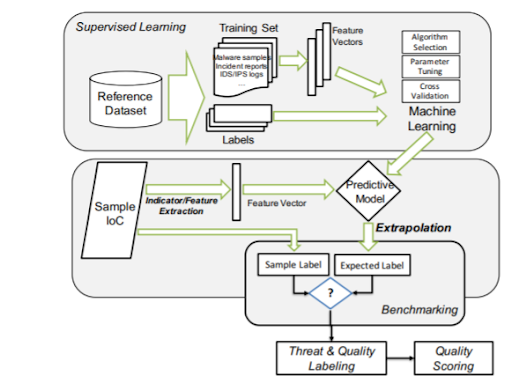
\includegraphics[width=1\linewidth]{Figures/co-relation}
    \caption{Co-relation process: Cyber news data}
    \label{fig:co-relation}
\end{figure}


\subsection{Analytics}
With the growing inflow of cyber newsfeed data 
and due to lack of cyber security professional performing analysis 
on the cyber newsfeed data, 
advanced analytics is gaming prominence 
and can be used in the consolidation process in order to simplify the mass of collected data \citep{dull2015cyberthreat}. 
In order to support the complexity of data structures 
of the cyber domain, 
the system should support, association, aggregation, composition and generalization \citep{brown2015cyber}. 
This domain is quite mature and literature suggest that 
big data architectures 
can be used to perform real-time network traffic processing, distributed messaging and scalable data storage. 
Then, the cyber professionals can focus on effective cyber threat intelligence analytics, 
rather than being hindered by data management, aggregation, reconciliation and formatting \citep{wheelus2016towards}. 

Automated and advanced Analytical capabilities of cyber threat intelligence platforms are mostly licensed and not available under open source distribution \citep{sauerwein2017threat}.

\section{Conclusion}
This concludes my literature work on the existing knowledge available for the current state of available artefacts mainly including people, processes and activities. This knowledge would be applied to the create the new artefact \enquote{Cybernewsfeed Technology}.


